\chapter{Methodology}
\label{cp:methodology}
\section{Apparatus}

In this experiment, we calibrated the low-speed wind tunnel at Iowa State University, the test section of which is shown in \autoref{fig:test_section}.

\begin{figure}[htpb]
    \centering
    \includegraphics[width=0.75\linewidth]{Figures/test_section.jpeg}
    \caption[Photograph of the test section in the low-speed wind tunnel]{Photograph of the test section in the low-speed wind tunnel at Iowa State University.}
    \label{fig:test_section}
\end{figure}

The remote shown in \autoref{fig:remote} is used to control the frequency of the motor that forces air through the closed-loop wind tunnel. To calibrate the wind tunnel and establish a relationship between the frequency of the motor and the dynamic pressure (or velocity) in the test section, a pitot tube was inserted into the middle of the test section, as shown in \autoref{fig:pitot_tube}. Additionally, two tubes were connected to the static pressure ports at points A and E in the test section. These points are denoted in \autoref{fig:lab_drawing} and shown in \autoref{fig:static_pressure_ports}.

\begin{figure}[htpb]
    \centering
    \includegraphics[angle=-90, width=0.25\linewidth]{Figures/remote.jpeg}
    \caption[Photograph of the wind tunnel remote]{Photograph of the remote that is used to control the low-speed wind tunnel.}
    \label{fig:remote}
\end{figure}

\begin{figure}[htpb]
    \centering
    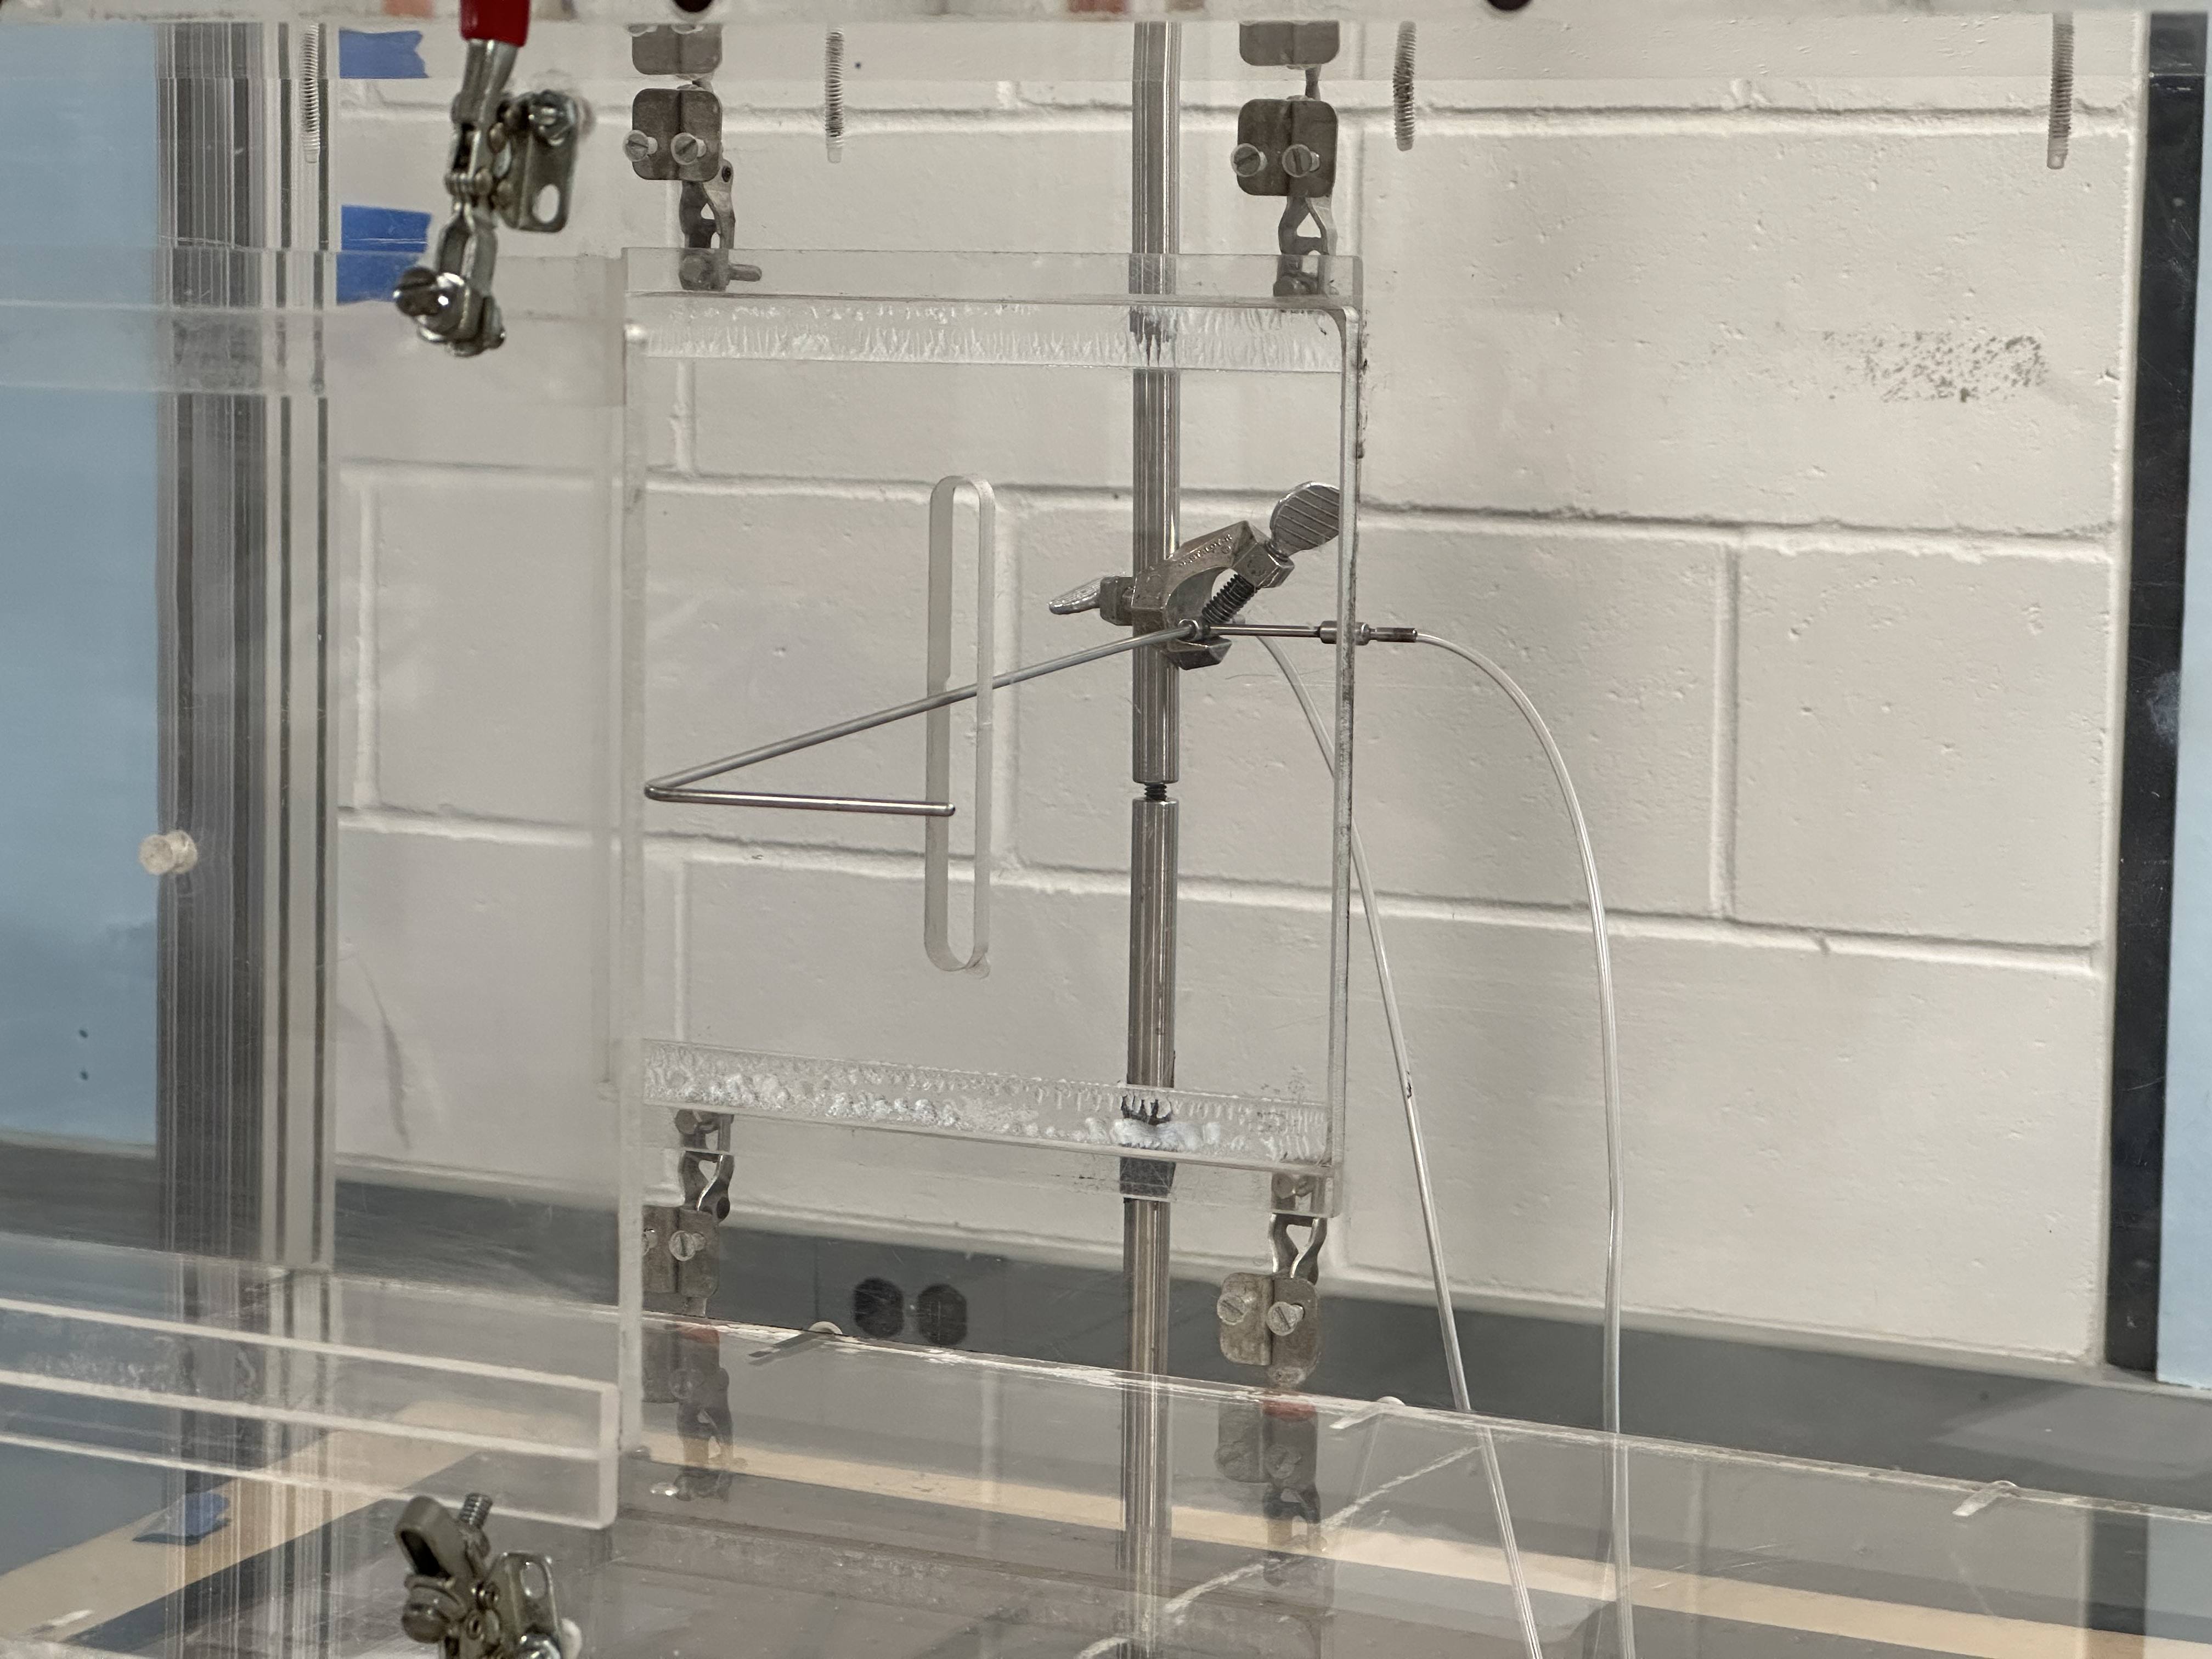
\includegraphics[width=0.6\linewidth]{Figures/real_pitot_tube.jpeg}
    \caption[Photograph of the pitot tube in the wind tunnel]{Photograph of the pitot tube used to calibrate the wind tunnel.}
    \label{fig:pitot_tube}
\end{figure}

\begin{figure}[htpb]
    \centering
    \includegraphics[width=0.5\linewidth]{Figures/static_pressure_ports.jpeg}
    \caption[Photograph of static pressure ports]{Photograph of the static pressure ports at points A and E.}
    \label{fig:static_pressure_ports}
\end{figure}

Four tubes are connected from the wind tunnel to the manometer shown in \autoref{fig:manometer}. These tubes indirectly measure the

\begin{itemize}
    \item static pressure at point A,
    \item static pressure at point E,
    \item total—or stagnation—pressure in the pitot tube, and
    \item static pressure in the pitot tube.
\end{itemize}

\noindent{}Additionally, there are a number of tubes not connected to the wind tunnel which are used to measure the reference pressure in the lab. Each graduation marking on the manometer denotes a tenth of an inch.

\begin{figure}[htpb]
    \centering
    \includegraphics[width=0.75\linewidth]{Figures/water_manometer.jpeg}
    \caption[Photograph of the manometer]{Photograph of the manometer used to measure the pressure at different points in the wind tunnel.}
    \label{fig:manometer}
\end{figure}

\section{Test Procedure}
To determine the relationship between the dynamic pressure in the test section and the static pressure differential at points A and E, we measured the heights of each active tube in the manometer for a number of different motor frequencies. This is the procedure we followed:

\begin{enumerate}
    \item With the wind tunnel motor turned off, measure and record the height of the liquid in each active tube and the reference tube.
    \item Increase the motor frequency by \qty{5}{\hertz} and wait for the liquid in the manometers to stabilize. \label{step:increase_freq}
    \item Record the new heights of the liquid in each active tube and the reference tube. \label{step:record_heights}
    \item Repeat \autoref{step:increase_freq} and \autoref{step:record_heights} for frequencies \qtyrange{5}{40}{\hertz}.
\end{enumerate}

\noindent{}The data collected from these steps are recorded in \autoref{tab:raw_data}.

\section{Derivations}

From the lab two manual, we are given

\begin{equation}\label{eq:dynamic_pressure_relationship}
    \Delta{}P = Cq_t
\end{equation}

\noindent{}where \gls{DeltaP} is the static pressure differential between points A and E, \gls{C} is a dimensionless constant, and \gls{q_T} is the dynamic pressure of the test chamber \citep{lab2-manual}. \autoref{eq:dynamic_pressure_relationship} can then be rearranged to

\begin{equation}\label{eq:dynamic_pressure_relationship-2}
    q_T = \frac{1}{C}\Delta{}P
\end{equation}

\noindent{}Since the calibration constant, \gls{K}, is defined as

\begin{equation}\label{eq:K_def}
    K = \frac{1}{C}
\end{equation}

\noindent{}we can substitute \autoref{eq:K_def} into \autoref{eq:dynamic_pressure_relationship-2} to get

\begin{equation}\label{eq:dynamic_pressure_relationship-3}
    q_T = K\Delta{}P
\end{equation}

\subsection{Quantifying Dynamic Pressure}\label{sec:quantify_dynamic_pressure}

To find \gls{K}, we must first use the data collected from the experiment to calculate \gls{q_T} and \gls{DeltaP}. To quantify \gls{q_T}, we start by using the equation of total pressure,

\begin{equation}\label{eq:total_pressure}
    P_0 = P + q
\end{equation}

\noindent{}where \gls{P_0} is the total or stagnation pressure, \gls{P} is the static pressure, and \gls{q} is the dynamic pressure. From \autoref{eq:total_pressure}, we can derive an expression for \gls{q_T}:

\begin{equation}\label{eq:dynamic_pressure_test_chamber}
    q_T = P_{0,T} - P_T
\end{equation}

\noindent{}where \gls{P_0T} is the total pressure in the test chamber and \gls{P_T} is the static pressure in the test chamber \citep{lab2-manual}.

\gls{P_0T} and \gls{P_T} were measured indirectly using a manometer. From the lab manual, we are given the following manometer equation:

\begin{equation}\label{eq:manometer}
    P = P_{ref} - \rho_{water} g \left(H - H_{ref}\right)
\end{equation}

\noindent{}where \gls{P} is the pressure being measured, \gls{P_ref} is the reference pressure, \gls{rho_water} is the density of water, \gls{g} is the acceleration due to gravity, \gls{H} is the height of the water in the active manometer tube, and \gls{H_ref} is the height of the water in the reference manometer tube \citep{lab2-manual}. Using \autoref{eq:manometer}, we can define expressions for \gls{P_0T} and \gls{P_T}:

\begin{align}
    P_{0,T} &= P_{ref} - \rho_{water} g \left(H_{total} - H_{ref}\right) \label{eq:total_pressure_manometer} \\
    P_T &= P_{ref} - \rho_{water} g \left(H_{static} - H_{ref}\right) \label{eq:static_pressure_manometer}
\end{align}

\noindent{}where \gls{H_total} is the height of the water in the manometer tube connected to the total pressure port of the pitot tube and \gls{H_static} is the height of the water in the manometer tube connected to the static pressure port of the pitot tube.

Substituting \autoref{eq:total_pressure_manometer} and \autoref{eq:static_pressure_manometer} into \autoref{eq:dynamic_pressure_test_chamber}, we can simplify the expression for \gls{q_T} as follows:

\begin{align}
    q_T &= \left[P_{ref} - \rho_{water} g \left(H_{total} - H_{ref}\right)\right] - \left[P_{ref} - \rho_{water} g \left(H_{static} - H_{ref}\right)\right] \nonumber \\
    &=-\rho_{water}gH_{total}+\rho_{water}gH_{static} \nonumber \\
    &=\rho_{water}g\left(H_{static} - H_{total}\right) \label{eq:dynamic_pressure_final}
\end{align}

\noindent{}\autoref{eq:dynamic_pressure_final} was used in our \acrfull{matlab} script (see \autoref{cp:code}) to calculate \gls{q_T} for each of the motor frequencies we tested.

\subsection{Quantifying the Static Pressure Differential}

An equation for the static pressure differential, \gls{DeltaP}, can be derived in a similar fashion to \gls{q_T}. For more details see \autoref{sec:quantify_dynamic_pressure}. Furthermore, the equation for \gls{DeltaP} is

\begin{equation}\label{eq:pressure_diff_final}
    \Delta{}P = \rho_{water}g\left(H_E - H_A\right)
\end{equation}

\noindent{}where \gls{H_E} is the height of the water in the manometer tube connected to the static pressure port at point E and \gls{H_A} is the height of the water in the manometer tube connected to the static pressure port at point A. \autoref{eq:pressure_diff_final} was used in our \acrshort{matlab} script to calculate \gls{DeltaP} for each of the motor frequencies we tested.

\subsection{Determining the Calibration Constant}\label{sec:determine_calibration_constant}

Once we calculated the values of \gls{q_T} and \gls{DeltaP} for each of the motor frequencies, we used \acrshort{matlab} to plot \gls{q_T} vs. \gls{DeltaP} (see \autoref{fig:dynamic_pressure_graph}). We used the \verb|polyfit()| function to calculate the coefficients of a linear line of best fit. Since \gls{K} is the slope of \autoref{eq:dynamic_pressure_relationship-3}, it follows that the slope of the line of best fit is approximately \gls{K}.

\subsection{Calculating the Test Chamber Velocity}\label{sec:calc_velocity}

Since we have already calculated the values of \gls{q_T} at for each of the motor frequencies we tested, we can use \autoref{eq:dynamic_pressure} to derive an expression for the velocity of the test chamber:

\begin{equation} \label{eq:velocity}
    v_T = \sqrt{\frac{2q_T}{\rho_{air}}}
\end{equation}

\noindent{} where \gls{v_T} is the velocity of air in the test chamber and \gls{rho_air} is the density of air. Using \autoref{eq:velocity} and our \acrshort{matlab} script, we calculated the velocity of air in the test chamber for each of the motor frequencies and created a plot of test chamber airspeed vs. motor frequency (see \autoref{fig:velocity_graph}). Finally, we used the \verb|polyfit()| function once more to calculate a linear line of best fit for the velocity vs. motor frequency relationship.